\chapter{Conclusion}
\label{chap:conclusion}

In conclusion, the implementation of a Python routine for complete automation and integration of the system has improved the precision of experiments and enabled real-time collection of extensive data without requiring the expertise and time of a specialized scientist. 
This project underscores the potential of automation in enhancing scientific research and accelerating progress towards achieving research goals.
In addition to its potential in scientific research, the software developed in this project can also be leveraged by industrial approaches. 
Furthermore, the classification methods and system control implemented in this project have yielded promising results and can be further optimized in the future. Overall, this project serves as a contribution towards the advancement of automated systems and the optimization of experimental processes.

\section{Proposal for continuation}

To continue, my proposal would be to prioritize the improvement of the classification step. 
Ideally, we could use machine learning or another algorithm to ensure accurate classification with a broad range of liquids.
By achieving a reliable classification, we can then implement more effective controller logic or approaches. 
In this regard, I would like to present the concept of a fuzzy controller as a potential solution.

\subsection{Machine Learning}

    When it comes to classifying spraying modes, machine learning represents a sophisticated and trendy approach.
    This project was designed in order to substitute our statistical classifier for a more general and accurate algorithm.
    
    The data collected in this project was saved in 0.5s samples together with its classification allowing it to be used for supervised learning.
    Experimental trials were conducted to explore machine learning algorithms to classify the data. Unfortunately, despite efforts, an accurate method of distinguishing between classifications could not be identified.

\subsection{Fuzzy Controller}

        One challenge in implementing the controller in this project is that we don't have a real value as feedback, instead, the feedback from the controller loop is a classification, which makes it difficult to apply many of the principles of control theory that are designed for continuous control. 
        As this project involves logical control, it requires a different approach. 
        
        The controller project that will be presented is an attempt to quantify the classification and fit it in a fuzzy control model.
        That approach is for an open loop control system and the input and outputs of the controller must be fuzzyfied.

        Firstly, the fuzzyfication and defuzzyfication machines were implemented using the data acquired in the experiment of step routine\ref{subsec:step_routine}, mapping the area of each spraying mode according to its potential.
        Figure \ref{fig:fuzzyy} shows the steps of fuzzyfication and defuzzyfication within the input and output of the controller.


            \begin{figure}[H]
                \centering
                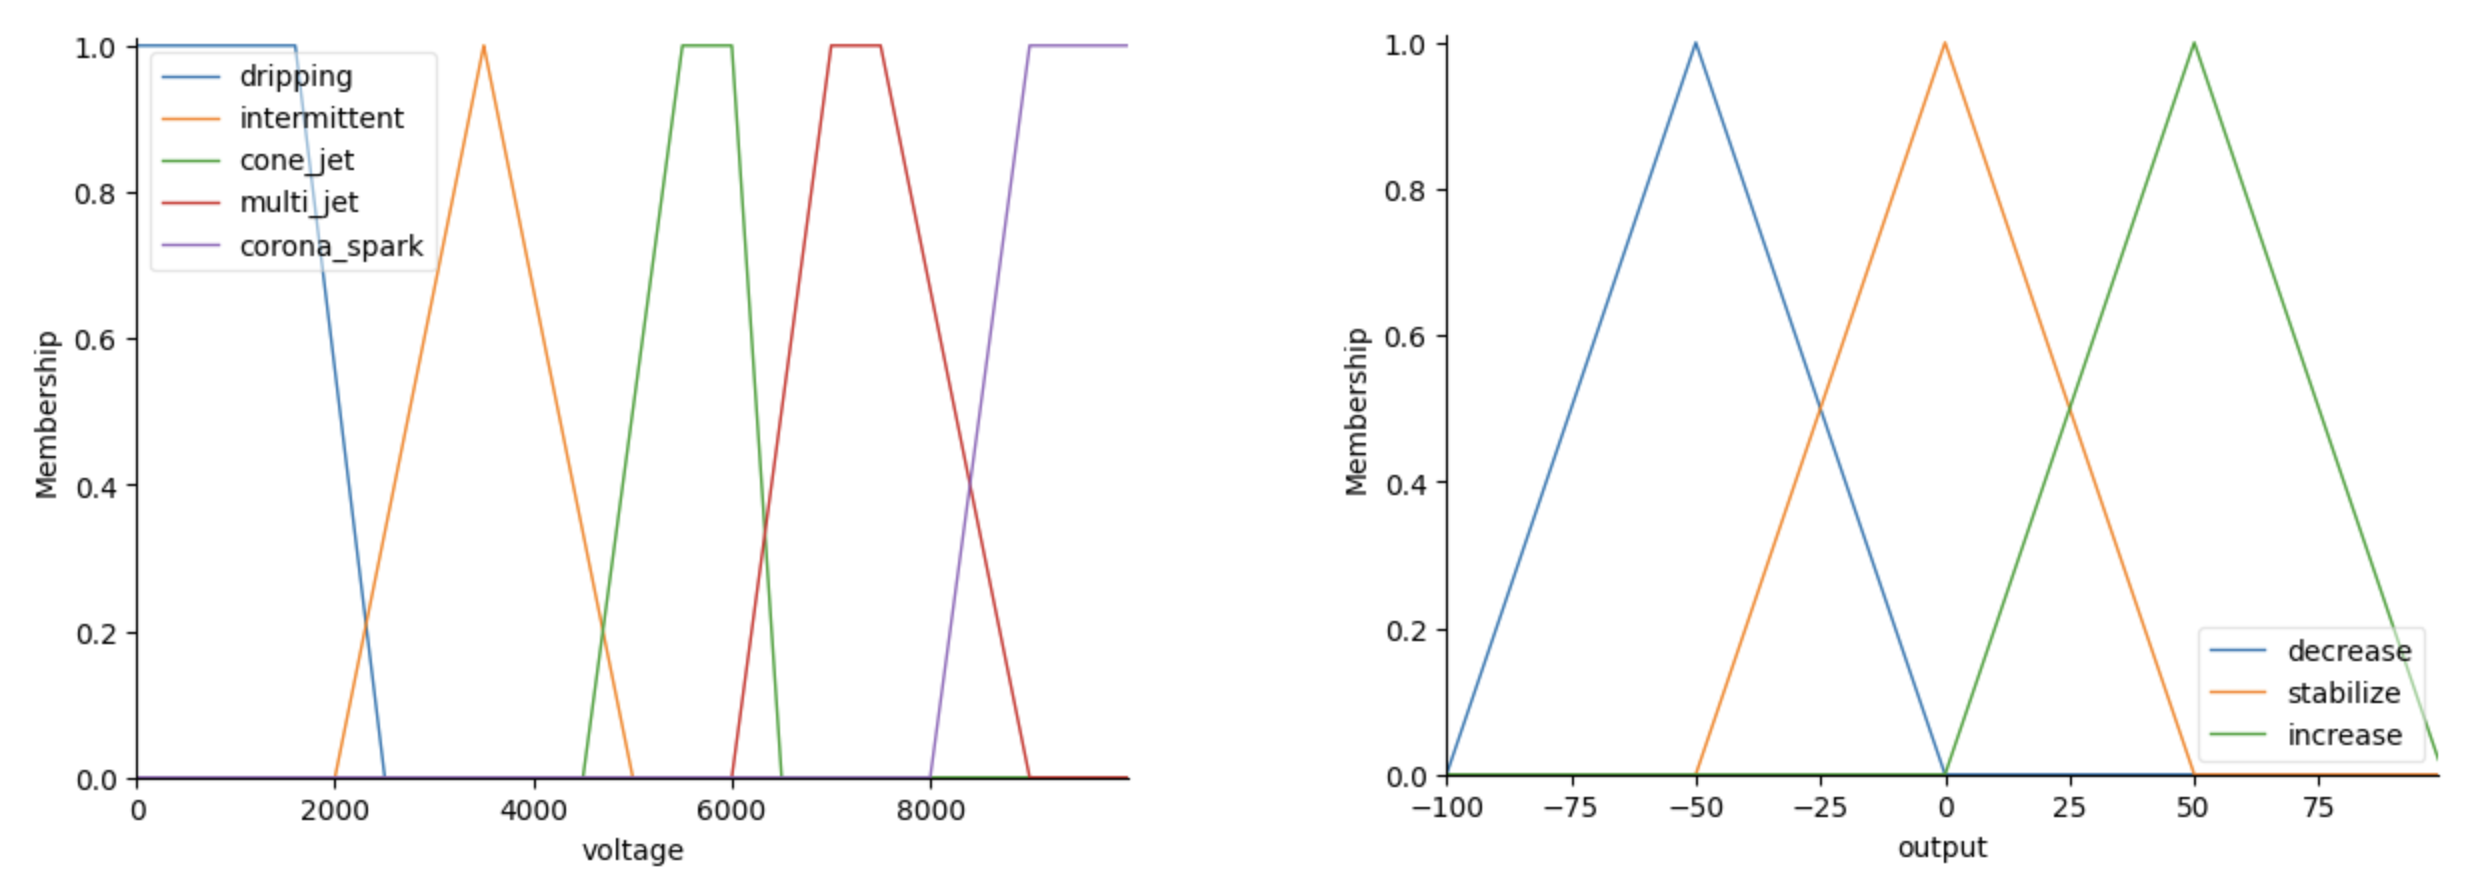
\includegraphics[width=17cm]{Figuras/fuzzy/Fuzzyy.png}
                \caption{fuzzyfication of input and defuzzyfication of output.}
                \label{fig:fuzzyy}
            \end{figure}



        Our controller is an algorithm that calculate the output with a geometrical calculus on the membership functions of the input and output according to our rules listed below.

        Fuzzy Rules:

        -> IF dripping THEN increase

        -> IF intermittent THEN increase

        -> IF cone jet THEN stabilize

        -> IF multi jet THEN decrease

        -> IF corona THEN decrease


        In figure \ref{fig:fuzzyy1}, two tests were made. Test 1 with a higher voltage of 7000V accusing it to be 100\% in multi jet and the output of decrease voltage. Test 2 shows the opposite case when the voltage is lower than expected.

    \begin{figure}[H]
        \centering
        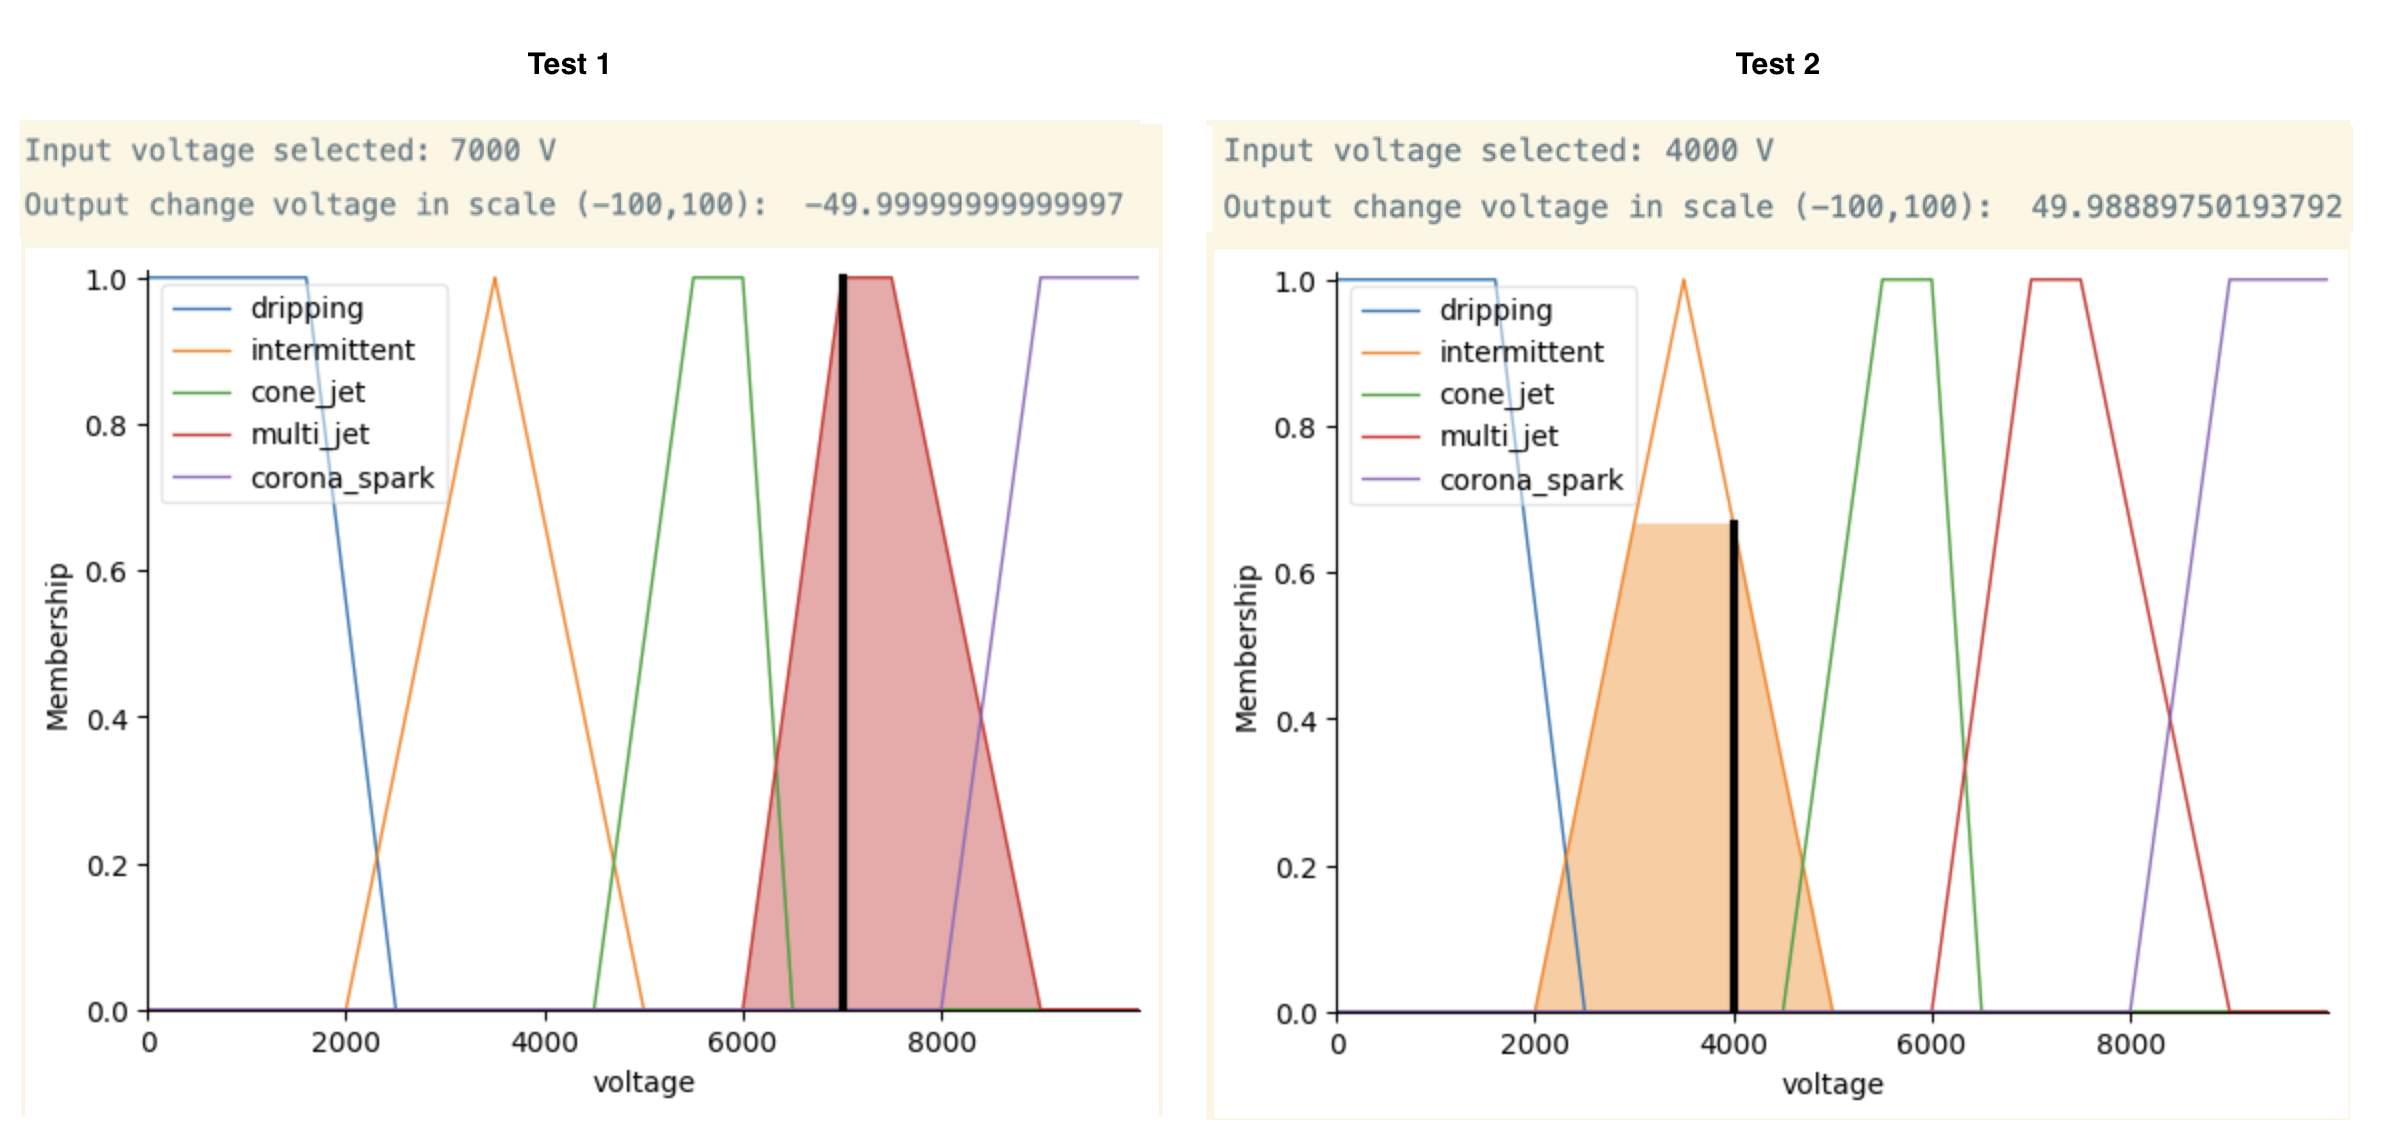
\includegraphics[width=17cm]{Figuras/fuzzy/test3.png}
        \caption{Test implemented to validate the concept of fuzzy controller in this project.}
        \label{fig:fuzzyy1}
    \end{figure}
        

    \section{Final Discussions}

        The works presented in this report represent a continuation and refinement of previous efforts to develop a more precise and versatile automation routine that can be effectively applied in both industrial and research applications. 
        
        The previous student work focused on predicting corona streamers or spark discharges\cite{Monica} and her automation routine provided a valuable proof-of-concept. 
        
        The current project builds on this foundation and highlights several key results, including the integration of a liquid pump into the software and the development of a routine that can be easily modeled to fit a control model, making it straightforward to implement new control algorithms or experiment routines. 
        The software was also remodeled to support threads, allowing for the separation of each subsystem and the exchange of data between them using queue data structures. A classification for multi-jet spraying mode was developed, along with a simple controller to demonstrate proof of concept. 
        Additionally, the saving of data was optimized to a real-time streaming format and expanded to include more sensor data. Finally, the algorithm usability was restructured to make it more intuitive for users through the use of a setup file.

        
\clearpage
